% Created 2020-12-26 Sat 19:42
% Intended LaTeX compiler: pdflatex
\documentclass[11pt]{article}
\usepackage[utf8]{inputenc}
\usepackage[T1]{fontenc}
\usepackage{graphicx}
\usepackage{grffile}
\usepackage{longtable}
\usepackage{wrapfig}
\usepackage{rotating}
\usepackage[normalem]{ulem}
\usepackage{amsmath}
\usepackage{mathbbol}
\usepackage{textcomp}
\usepackage{amsmath}
\usepackage{amsfonts}
\usepackage{capt-of}
\usepackage{hyperref}
\usepackage{bm}
\date{\today}

\hypersetup{
 pdfauthor={Rui Ying},
 pdftitle={Principal Component Analysis},
 pdfkeywords={PCA},
 pdfsubject={Statistic},
 pdfcreator={Emacs 27.1 (Org mode 9.4.2)}, 
 pdflang={English}}
\begin{document}

%\tableofcontents

\section{Definition of covariance matrix}
\indent

Suppose \textbf{X} is a d-dimensional random vector (with d random variables), and \bm{$X_1$},\dots,\bm{$X_n$} is n independent copies of \textbf{X}.

Write $\bm{X_i} = (X_i^1,\dots,X_i^d)^T$, the subscript means the $i_{th}$ copy, the superscript means the number of random variable (i.e. scala). %Then we can combine all the $\bm{X_i}$ together as a new matrix, $\mathbb{X}$ (n by d).

\begin{align}
  \bm{X} =
  \begin{pmatrix}
    X^1\\
    X^2\\
    \dots \\
    X^d
  \end{pmatrix}
  %
  %\mathbb{X} =
  %\begin{pmatrix}
  %  \dots & \bm{X_1}^T & \dots\\
  %  \dots & \bm{X_2}^T & \dots\\
  %  \dots & \bm{X_3}^T & \dots
  %\end{pmatrix}
\end{align}

Then we can know the covariance matrix, which means take two different scalas or coordinates (notice the superscript) from a vector and compute their covariance. For convenience, not use bold X again as before.
\begin{align}
  \Sigma & = cov(X^i,X^j)\\
         & = \mathbb{E}(XX^T)-\mathbb{E}(X)\mathbb{E}(X)^T\\
         & = \mathbb{E}[(X-\mathbb{E}(X))(X-\mathbb{E}(X))^T]
\end{align}
When it comes to empirical data, we use average $\bar{X}$ to replace expectation\footnote{Here can be a little comfused because in we used subscript before but here we have $X_i$. This is because in theory, $E(X^1)$ is the expectation of random variable $X^1$, but empirically we sampled many times and calculate their average} and use the empirical covariance matrix \textbf{S} to replace the $\Sigma$), 

\begin{align}
  \mathbb{E}(X) & =
  \begin{pmatrix}
    \mathbb{E}(X^1)\\
    \vdots\\
    \mathbb{E}(X^d)
  \end{pmatrix}
  \rightarrow
  \begin{pmatrix}
    \frac{\sum}{n} X_i^1\\
    \vdots\\
    \frac{\sum}{n} X_i^d\\
  \end{pmatrix}\\  
  S &= \frac{1}{n}\sum (X_iX_i^T) - \bar{X}\bar{X}^T \label{eq6}
\end{align}

In order to eliminate the sum character, we multiply a $\mathbb{1}$ to replace the average. $\mathbb{1}=(1,\dots,1)^T$
\begin{align}
  &\bar{X} = \frac{1}{n}\sum X_i \;\;\;\;\;\;
  \mathbb{X} =
  \begin{bmatrix}
    \vdots&\vdots&\vdots\\
    X_1&X_2&X_n\\
    \vdots&\vdots&\vdots
  \end{bmatrix}\\
  &\frac{1}{n}\mathbb{X}^T\mathbb{1}=\frac{1}{n}\sum X_i = \bar{X}
\end{align}
And we can see that
\begin{align}
  M_i &=
  \begin{bmatrix}
    0&\vdots & 0& 0\\
    0&X_i &0&0\\
    0&\vdots&0&0\\
  \end{bmatrix}\\
  \mathbb{X}^T \mathbb{X} &= \sum_i^n M_iM_i^T = \sum_i^nX_iX_i^T\\
  \mathbb{X}^T &= M_1 + M_2 + \dots + M_n
\end{align}

Then in Eq.6 can be transformed into
\begin{align}
  S = & \frac{1}{n}\mathbb{X}^T\mathbb{X} - \frac{1}{n^2}\mathbb{X}^T(\mathbb{1}\mathbb{1}^T)\mathbb{X}\\
  = & \frac{1}{n}\mathbb{X^T}(I_d - \frac{1}{n}\mathbb{1}\mathbb{1}^T)\mathbb{X}\\
  = & \frac{1}{n}\mathbb{X}^TH\mathbb{X}
\end{align}

So, obviously matrix $H$ is a prthogonal projector (you can proof by calculate $H^TH$), what's the subspace this projector project a vector to?
\begin{align}
  H & = (I_d - \frac{1}{n}\mathbb{1}\mathbb{1}^T)\\
& = \begin{bmatrix}
  1-\frac{1}{n} & \cdots & \frac{1}{n}\\
  \vdots & \ddots & \vdots\\
  \frac{1}{n} & \cdots & 1-\frac{1}{n}  
\end{bmatrix} 
\end{align}
so for any vector $\bm{v}$, we have
\begin{align}
  H\bm{v} & = \bm{v} - \frac{1}{n}(\bm{v}^T\mathbb{1})\mathbb{1}\\
    & = \bm{v} - \bar{\bm{v}}\mathbb{1}
\end{align}
which means a vector minus its means by all elements. And it's clear that
\begin{align}
  avg(H\bm{v}) = 0
\end{align}
means $H$ projects vector $\bm{v}$ to the subspace that has the mean of 0. Or in another words, Hv $\perp$ span of $\mathbb{1}$ because $(Hv)^T\mathbb{1} = 0$.

\section{Core: $u^T\Sigma u$}

Take a vector $\bm{u} \in \mathbb{R}^d$ (column vector), then
\begin{align}
  u^T\Sigma u & = u^T[E(XX^T) - E(X)E(X)^T]u\\
  & = E[(u^TX)(X^Tu)] - E(u^TX)E(X^Tu)\\
  & = E[(u^TX)^2] - [E(u^TX)]^2\\
  & = var(u^TX)
\end{align}

The transition to Eq.22 is because $u^TX = X^T$ = a number.
So this is the magic now, the covariance matrix is equal to the variance of $u^TX$. What's is $u^TX$?

$u^TX$ is the the inner product betwen u and X. Look at my handnote,in geometric, it means the length of red line. So with multiple points, the variance means \emph{the degree of dispersion along the vector u}.

\begin{figure}[hb!]
  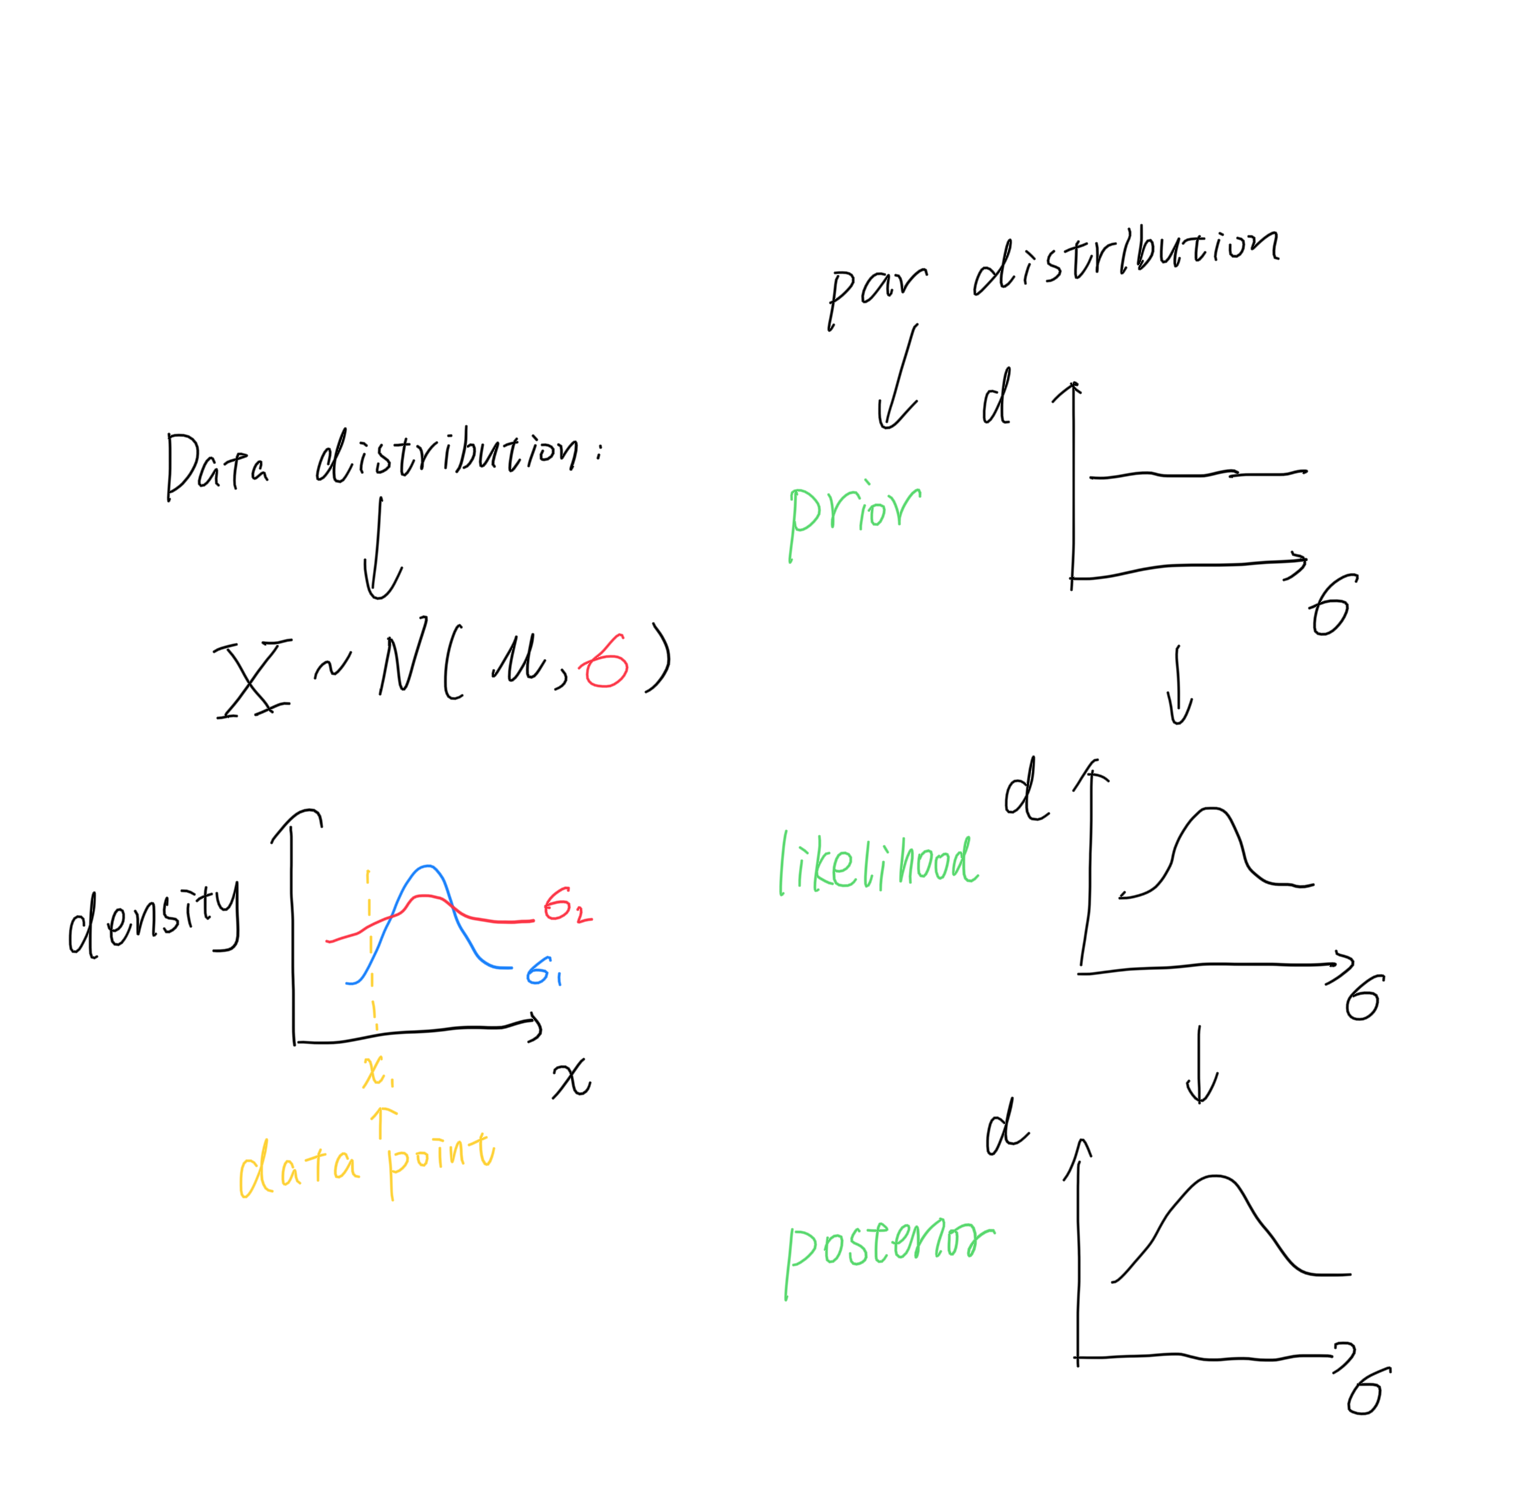
\includegraphics[scale=0.3]{handnote.PNG}
\end{figure}

Therefore, we need to find the vector $\bm{u}$ to maxmize our variance, because we reduce the dimension but don't want to lose too much information (image a 3D olive, we cut it and wanna get the cross section with as long and wide as possible).

\section{Spectral decomposition/Eigendecomposition}
\subsection{Variance is eigenvalue}
Since $\Sigma$ and S are symmetric, we can decompose it into this form:
\begin{align}
  \Sigma = PDP^{T} \; (or PDP^{-1})
\end{align}
We know that matrix P consists of all eigenvectors of $\Sigma$, and 
\begin{align}
  \Sigma v_1 = PDP^Tv_1=\lambda_1v_1\\
  v_1^T\Sigma v_1 = \lambda_1v_1^Tv_1=\lambda_1
\end{align}
Therefore, the variance along eigenvectors(here $v_1$ means the first and largest eigenvector) is simply the eigevalue $\lambda$.

Assume $\bar{X}=0$ to ensure $\bar{X}\bar{X}^T=0$ and make calculation easier, the Equation \ref{eq6} becomes
\begin{align}
  S=\Sigma X_i X_i^T
\end{align}

\subsection{Another way to proof}

Suppose %$\lambda_i$ are ordered by number (i.e. $\lambda_1 > \lambda_2 > \dots > \lambda_n$)
$y_i=P^TX_i$ (which is the projected vector). Then
\begin{align}
  \bar{y_i} & = \overline{P^TX_i} = P^T\bar{X_i} = 0\\
  S^\prime & = \frac{1}{n}\sum y_iy_i^T\\
  &=\frac{1}{n}\sum (P^TX_i)(P^TX_i)^T\\
  &=\frac{1}{n}\sum (P^TX_iX_i^TP)\\
  &=\frac{1}{n}\sum (P^TSP)
\end{align}
And because $S=PDP^T$, we have
\begin{align}
  S^\prime &= P^T(PDP^T)P\\
  & = D
\end{align}
We know D is a diagonal matrix made up of eigevalue $\lambda_i$. So $cov(y^i,y^j)=0$ when $i\neq j$. In other words, $lambda_i = var(P^TX_i)$.

\subsection{Why eigenvector is best?}
\indent
Here we need to proof why eigenvectors are the ones make variance largest, because there're so many choices.

Suppose $b=P^Tu$ and $u$ is unit vector.
\begin{align}
  u^TSu = b^TDb=\sum_{j=1}^d \lambda_j b_j^2 \leq \sum_{j=1}^d \lambda_1 b_j^2 
\end{align}

$\lambda_1$ here still means the largest eigenvalue. So for any vector $u$, we can know that $\lambda_1$ is the largest variance and the Nth largest eigenvectors are called ($N_{th}$) Principal Components.

In extrme cases, if $n >> d$(much more data samples than dimension), then the empirical data converge to a consistent estimator (which means perfect). Otherwise, if $d >> n$, the angle between eigenvectors of $\Sigma$ and S will be very large (which means very bad estimator). And we need sparse PCA (I don't konw this either).


\end{document}